\documentclass[11pt]{article}

\usepackage[margin=1in]{geometry}
\usepackage{amsmath,amssymb,mathtools}
\usepackage{booktabs}
\usepackage{hyperref}
\usepackage{xcolor}
\usepackage{tikz}
\usetikzlibrary{arrows.meta,positioning,decorations.pathreplacing}

\title{How \texttt{genlasso.trendfilter.cv} Works in the 1D Benchmark}
\author{gflow metric-lowpass benchmark notes}
\date{\today}

\newcommand{\R}{\mathbb{R}}
\newcommand{\argmin}{\operatorname*{arg\,min}}

\begin{document}
\maketitle

\section{What is \texttt{genlasso.trendfilter.cv}?}

\texttt{genlasso.trendfilter.cv} is not an exported function from the
\texttt{genlasso} package. It is the benchmark label used in our report for the
following wrapper:
\[
\begin{array}{ll}
\text{solution path:} & \texttt{genlasso::trendfilter(y, pos = x, ord = 2)},\\[2mm]
\text{tuning:} & \texttt{genlasso::cv.trendfilter(fit, k = 5, mode = "lambda")},\\[2mm]
\text{final fit:} & \texttt{coef(fit, lambda = cv\$lambda.min)\$beta}.
\end{array}
\]
Thus the actual algorithm is \emph{quadratic trend filtering} with a
five-fold cross-validated choice of the regularization parameter
\(\lambda\).

The name ``lasso'' can be confusing here. In high-dimensional regression, the
ordinary lasso penalizes the absolute values of regression coefficients. Trend
filtering instead penalizes the absolute values of \emph{discrete derivatives}
of the fitted curve. The lasso idea is the same--an \(\ell_1\) penalty creates
sparsity--but the sparse objects are not selected covariates. They are selected
locations where the fitted curve is allowed to change curvature.

\section{The data and the fitted values}

Assume the observations are ordered by position:
\[
0 \le x_1 < x_2 < \cdots < x_n \le 1,
\qquad
y_i = f(x_i) + \varepsilon_i.
\]
Trend filtering estimates the vector of fitted values
\[
\theta = (\theta_1,\ldots,\theta_n)^T,
\qquad
\theta_i \approx f(x_i).
\]
It does not first choose knots and then fit a spline. Instead, it estimates the
values \(\theta_i\) directly, while penalizing changes in discrete derivatives.

\section{The basic optimization problem}

For polynomial order \(k\), trend filtering solves
\[
\widehat{\theta}_{\lambda}
=
\argmin_{\theta \in \R^n}
\left\{
\frac{1}{2}\sum_{i=1}^n (y_i-\theta_i)^2
+
\lambda \left\|D^{(k+1)}\theta\right\|_1
\right\}.
\]
Here:
\begin{itemize}
  \item The first term keeps the fitted values close to the noisy data.
  \item The second term penalizes roughness.
  \item \(D^{(k+1)}\theta\) is a vector of discrete \((k+1)\)st derivatives.
  \item The \(\ell_1\) norm,
  \[
  \left\|D^{(k+1)}\theta\right\|_1
  =
  \sum_j \left|(D^{(k+1)}\theta)_j\right|,
  \]
  encourages many of those discrete derivatives to be exactly zero.
\end{itemize}

In our benchmark, \(\texttt{ord}=2\), so \(k=2\). The fitted function is
therefore locally piecewise quadratic, and the penalty is on third-order
discrete differences:
\[
\widehat{\theta}_{\lambda}
=
\argmin_{\theta \in \R^n}
\left\{
\frac{1}{2}\sum_{i=1}^n (y_i-\theta_i)^2
+
\lambda \sum_{j=1}^{n-3}
\left|(D^{(3)}\theta)_j\right|
\right\}.
\]

\section{What do the differences mean?}

For equally spaced points, the first difference is
\[
(D^{(1)}\theta)_i = \theta_{i+1}-\theta_i.
\]
This measures local slope. The second difference is
\[
(D^{(2)}\theta)_i
=
\theta_{i+2}-2\theta_{i+1}+\theta_i.
\]
This measures local curvature. The third difference is
\[
(D^{(3)}\theta)_i
=
\theta_{i+3}-3\theta_{i+2}+3\theta_{i+1}-\theta_i,
\]
up to an irrelevant sign convention. This measures changes in curvature.

For \(\texttt{ord}=2\), the \(\ell_1\) penalty tries to make most third
differences zero. If the third difference is zero over a run of adjacent
points, then the fitted values over that run lie on a quadratic polynomial.
Where a third difference is nonzero, the curve can change quadratic piece.
Those locations behave like adaptively chosen knots.

\section{Why this is still lasso}

The ordinary lasso has the form
\[
\argmin_b
\left\{
\frac{1}{2}\|y-Xb\|_2^2+\lambda\|b\|_1
\right\}.
\]
It makes many entries of \(b\) exactly zero.

Trend filtering is a \emph{generalized lasso}:
\[
\argmin_{\theta}
\left\{
\frac{1}{2}\|y-\theta\|_2^2+\lambda\|D\theta\|_1
\right\}.
\]
Now the lasso penalty is applied after multiplying by a structured matrix
\(D\). In trend filtering, \(D=D^{(k+1)}\), so the sparse quantities are
discrete derivatives. Sparsity in derivatives means the fitted curve is simple
on long intervals and only changes shape at a limited number of data-adaptive
locations.

\section{Unequally spaced \(x\)-values}

Our benchmark samples \(x_i\) values randomly in \([0,1]\), so the gaps
\(x_{i+1}-x_i\) are not constant. The \texttt{genlasso} implementation supports
this through the \texttt{pos} argument. Internally, it replaces ordinary finite
differences by weighted finite differences, equivalent in spirit to divided
differences.

For first differences, the natural scaling is
\[
\frac{\theta_{i+1}-\theta_i}{x_{i+1}-x_i}.
\]
For higher orders, the package recursively builds a difference operator using
weights of the form
\[
\frac{m}{x_{i+m}-x_i},
\]
at derivative level \(m\). This adjusts the derivative penalty so that a large
gap in \(x\) is not treated the same way as a small gap.

The package documentation warns that arbitrary positions can be numerically
more delicate than equally spaced positions, especially for high polynomial
orders. Our wrapper uses \(k=2\), which is moderate: it allows curved fits but
does not go into the higher-order range where instability is more likely.

\section{The role of \(\lambda\)}

The tuning parameter \(\lambda\) controls the tradeoff between fidelity and
simplicity:
\[
\frac{1}{2}\|y-\theta\|_2^2
\quad\text{versus}\quad
\lambda\|D^{(3)}\theta\|_1.
\]

\begin{center}
\begin{tabular}{lll}
\toprule
\(\lambda\) & Effect on \(\theta\) & Interpretation\\
\midrule
very large & many third differences equal zero & very few knots, smooth simple curve\\
moderate & some nonzero third differences & adaptive piecewise quadratic curve\\
near zero & many nonzero third differences & curve follows data more closely\\
\bottomrule
\end{tabular}
\end{center}

Large \(\lambda\) says: ``Only bend the curve when the evidence is strong.''
Small \(\lambda\) says: ``Fit the observations more closely, even if that
requires many local bends.''

\section{Visual picture}

\begin{figure}[ht]
\centering
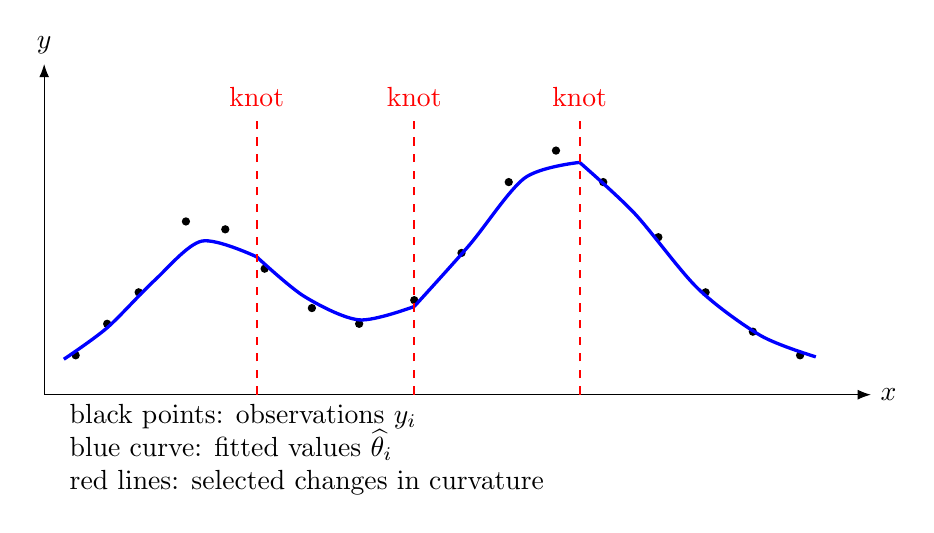
\begin{tikzpicture}[x=1cm,y=1cm,>=Latex]
  % axes
  \draw[->] (0,0) -- (10.5,0) node[right] {\(x\)};
  \draw[->] (0,0) -- (0,4.2) node[above] {\(y\)};

  % noisy points
  \foreach \x/\y in {0.4/0.5,0.8/0.9,1.2/1.3,1.8/2.2,2.3/2.1,2.8/1.6,
                    3.4/1.1,4.0/0.9,4.7/1.2,5.3/1.8,5.9/2.7,6.5/3.1,
                    7.1/2.7,7.8/2.0,8.4/1.3,9.0/0.8,9.6/0.5}
    \fill[black] (\x,\y) circle (1.5pt);

  % fitted curve, hand drawn as piecewise smooth segments
  \draw[blue,very thick]
    plot[smooth] coordinates {
      (0.25,0.45) (0.8,0.85) (1.4,1.45) (2.0,1.95) (2.7,1.75)
    };
  \draw[blue,very thick]
    plot[smooth] coordinates {
      (2.7,1.75) (3.3,1.25) (4.0,0.95) (4.7,1.12)
    };
  \draw[blue,very thick]
    plot[smooth] coordinates {
      (4.7,1.12) (5.4,1.9) (6.1,2.75) (6.8,2.95)
    };
  \draw[blue,very thick]
    plot[smooth] coordinates {
      (6.8,2.95) (7.5,2.3) (8.3,1.35) (9.1,0.75) (9.8,0.48)
    };

  % knots
  \foreach \x in {2.7,4.7,6.8}
    \draw[red,dashed,thick] (\x,0) -- (\x,3.55);
  \node[red] at (2.7,3.78) {knot};
  \node[red] at (4.7,3.78) {knot};
  \node[red] at (6.8,3.78) {knot};

  \node[align=left,anchor=west] at (0.2,-0.7) {
    black points: observations \(y_i\)\\
    blue curve: fitted values \(\widehat{\theta}_i\)\\
    red lines: selected changes in curvature
  };
\end{tikzpicture}
\caption{Quadratic trend filtering estimates fitted values at the observed
positions. Most third differences are zero, so the curve behaves like a
quadratic polynomial between selected knots.}
\end{figure}

\section{How cross-validation chooses \(\lambda\)}

\texttt{genlasso::trendfilter()} computes a solution path: a sequence of
\(\lambda\) values at which the fitted curve changes. Then
\texttt{genlasso::cv.trendfilter()} chooses among these candidate values.

For trend filtering, the package uses deterministic ordered folds rather than
random folds. Roughly, every \(k\)th interior point is assigned to the same
fold, while the first and last points remain in the training set. For a held
out point, the prediction is computed from neighboring fitted values. The
selected value
\[
\lambda_{\min}
=
\argmin_{\lambda}
\mathrm{CV}(\lambda)
\]
is the one with the smallest cross-validated prediction error.

In our benchmark, we use:
\[
k_{\mathrm{fold}} = 5,
\qquad
\texttt{mode = "lambda"},
\qquad
\lambda = \lambda_{\min}.
\]
Thus the method is allowed to adapt its smoothness separately for each
simulated dataset.

\section{Why it did so well in the 1D benchmark}

The benchmark truth is a smooth function on a one-dimensional interval, built
from mixtures of Gaussian bumps. Trend filtering is a strong method for exactly
this kind of problem because:
\begin{enumerate}
  \item It uses the true ordering of the data on the line.
  \item It adapts knot locations to the observed signal rather than placing
  knots uniformly.
  \item The \(\ell_1\) penalty allows local flexibility where the signal bends
  sharply, while keeping flatter regions simple.
  \item Cross-validation chooses the roughness level from the data.
\end{enumerate}

This also explains why the result is not a contradiction of the usual story
that lasso is useful in high-dimensional settings. The lasso mechanism is more
general than variable selection. Here it is being used for sparse changes in
the curve's derivatives.

\section{Relationship to the graph low-pass smoother}

The graph low-pass smoother estimates \(f\) by suppressing high-frequency
components of a graph Laplacian. On the path graph, this is also a kind of 1D
regularization, but the penalty is quadratic and spectral:
\[
\sum_i (y_i-f_i)^2 + \eta f^T L f
\]
or, after spectral filtering, an equivalent shrinkage of high-frequency
eigenvectors.

Trend filtering instead uses an \(\ell_1\) penalty on higher-order differences:
\[
\sum_i (y_i-\theta_i)^2 + \lambda \|D^{(3)}\theta\|_1.
\]
The distinction matters. Quadratic penalties tend to smooth everywhere.
\(\ell_1\) derivative penalties tend to smooth most places while allowing
localized bends. That localized adaptivity is a likely reason trend filtering
was so strong in the path-graph 1D benchmark.

\section{References}

\begin{itemize}
  \item Tibshirani, R. J. and Taylor, J. (2011). The solution path of the
  generalized lasso. \emph{Annals of Statistics}, 39(3), 1335--1371.
  \item Tibshirani, R. J. (2014). Adaptive piecewise polynomial estimation via
  trend filtering. \emph{Annals of Statistics}, 42(1), 285--323.
  \item Arnold, T. B. and Tibshirani, R. J. (2014). Efficient implementations
  of the generalized lasso dual path algorithm. arXiv:1405.3222.
  \item Kim, S.-J., Koh, K., Boyd, S. and Gorinevsky, D. (2009). \(\ell_1\)
  trend filtering. \emph{SIAM Review}, 51(2), 339--360.
\end{itemize}

\end{document}
